\chapterauthor{Tim Warburton}

\epigraph{ In the context of today’s CPU landscape, then, redesigning your application to run multithreaded on a multicore machine is a little like learning to swim by jumping into the deep end—going straight to the least forgiving, truly parallel environment that is most likely to expose the things you got wrong.}{Herb Sutter, The Free Lunch Is Over: A Fundamental Turn Toward Concurrency in Software}

\minitoc

\section{Introduction}
Up to this point in the course we have focused squarely on covering enough Linux/Terminal commands/emacs/Git/C/debugging tools so that you can begin to implement an algorithm and be relatively confident that your implementation will be correct. We have not focused on performance aspects for good reason. As Knuth so astutely said 

``\emph{The real problem is that programmers have spent far too much time worrying about efficiency in the wrong places and at the wrong times; premature optimization is the root of all evil (or at least most of it) in programming}'', Donald Knuth, \cite{knuth1974computer}.

However, Knuth wrote this in 1974 and in the intervening 45 years there has been an ongoing technological arms race in computer processor architecture that obliges us to pay attention to performance. It might help to understand the context of Knuth's comments by reviewing the timeline at \href{https://www.computerhistory.org/timeline/1974/}{computerhistory.org}. The Scelbi 8H computer introduced that year was based on an \href{https://en.wikipedia.org/wiki/Intel_8008}{Intel 8008} central processing unit (CPU). The Intel 8008 was an 8-bit CPU with a clock speed frequency of 0.5MHz and was fabricated with a 10 $\mu m$ manufacturing process. According to the Intel 8008 \href{https://en.wikipedia.org/wiki/Intel_8008}{wiki page} it could execute between 30,000 and 80,000 operations per second and was a purely sequential processor (one operation at a time). To get the most out of this CPU required super close attention to machine code implementations and algorithmic tuning. Doing this na\"{i}vely would likely result in a lot of headaches from introducing bugs in intricate code,hence Knuth's lament. 

We can contrast the Intel 8008 from 1974 with a top of the range Intel processor the \href{https://en.wikichip.org/wiki/intel/xeon_platinum/8180}{Intel Xeon Platinum 8180} introduced in 2017. This CPU is a 64-bit processor with a variable clock frequency that runs at approximately 2.3GHz (2.3 billion cycles per second) and is fabricated with a 14 $nm$ manufacturing process. A \href{https://software.intel.com/en-us/forums/software-tuning-performance-optimization-platform-monitoring/topic/761046}{back of the envelope calculation} estimates that this CPU can execute up to approximately 2 TFLOPS/s (2 trillion double precision floating point operations per second). This CPU is running with a clock speed 4600 times higher than the Intel 8008 (2300MHz/0.5MHz) but is capable of computing 66 millions as many operations per second (2e12 FLOPS/s / 3e5 OPS/s). The actual performance ratio is much higher since the Xeon 8180 is doing 64-bit floating point operations and the  8008 performance is based on 8-bit operations. So how can a CPU that has an instruction clock frequency that is only 4600 times higher perform 66 million times as many operations per second ? The important stat to pay attention to is the manufacturing process used for each CPU is radically different in scale. The silicon components have shrunk from 10$\mu m$ to 14$nm$. If all on-chip components shrank equally there could be 500,000 as many components on the new Intel CPU and they are simultaneously executing operations at a considerably higher clock frequency.

Knuth's observation has been commonly used as rationale to avoid optimizing code while blithely ignoring that key ``premature'' qualifier. However, today to squeeze reasonably optimal performance out of a modern CPU requires us to understand some of the architectural features that can be exploited by programmers. So we must talk about hardware aware optimization.  Since clock frequencies are no longer increasing as they did for much of the 70s and up until 2005 we are obliged to occupy the billions of CPU transistors by executing not one but multiple tasks at the same time.

Most modern CPUs are not monolithic sequential processors. Instead the CPU silicon is partitioned into multiple compute ``cores''. The Intel Xeon 8180 CPU for example has 28 physical cores (and that literally means the silicon is split into 28 actual compute units). Each of these compute cores itself is not a sequential processor. Instead it has multiple execution engines including integer arithmetic logic units (ALUs) and vector floating point units (FPUs). The vector FPUs are sometimes referred to as Single Instruction Multiple Data (SIMD) units. A modern SIMD unit can apply a single arithmetic operation on a vector of data of say 4,8, or 16 values per vector in small number of CPU clock cycles. 

There is much more information about the Intel Skylake class of CPUs including the 8180 at \href{https://en.wikichip.org/wiki/intel/microarchitectures/skylake_(server)}{wikichip.org}. One striking aspect is that the 8180 CPU is listed at \$10,000 whereas lower end parts in the same family list at about \$200! Over time the price for the high end CPUs will decrease but there will very likely be a higher end CPU that will still demand such a high premium. 

\begin{figure}
    \begin{center}
    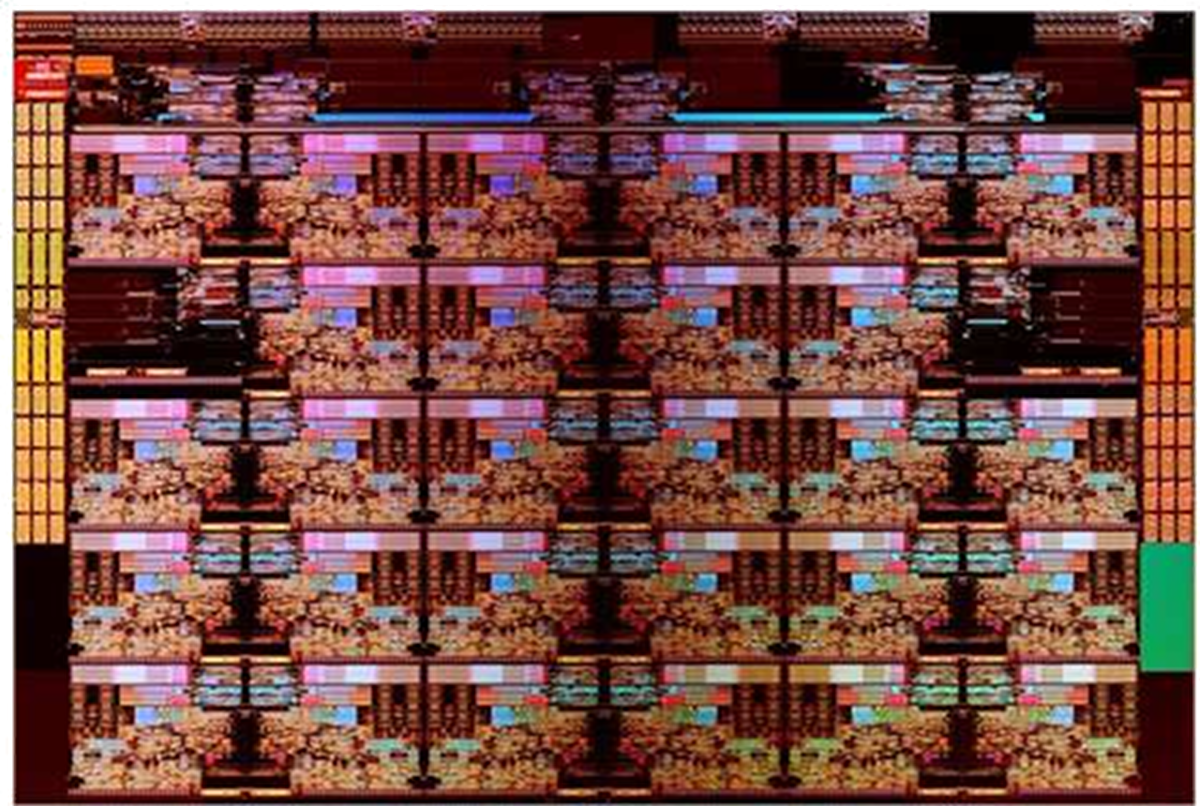
\includegraphics[width=0.8\linewidth]{figures/L14/skylakespxccdieshot.png}
    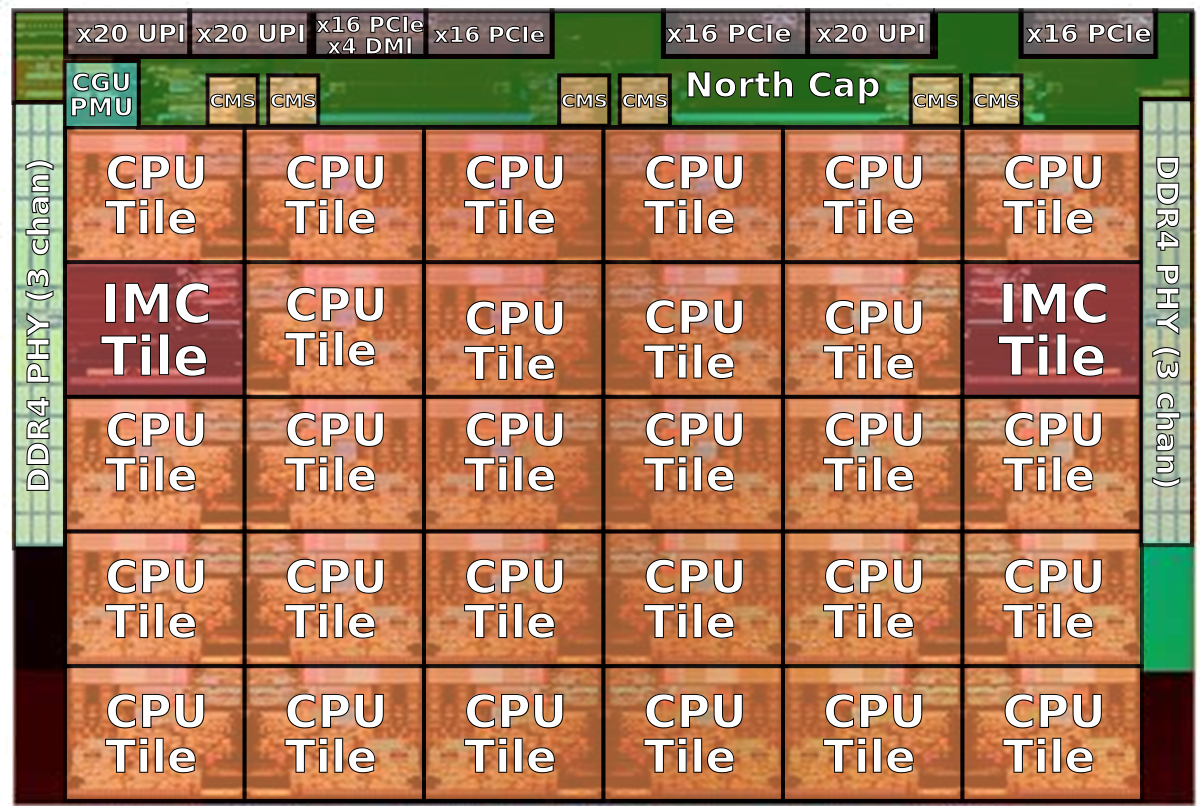
\includegraphics[width=0.8\linewidth]{figures/L14/skylakespxccdieshotannotated.png}
    \end{center}
    \caption{Top: die shot of Intel Xeon 8180. Botttom: block annotated version. Each CPU core is  labelled as a ``CPU Tile''. The two integrated memory controllers are each labelled as IMC ``Tile''.  Images sourced from \href{https://en.wikichip.org/wiki/File:skylake-sp_xcc_die_shot.png}{https://en.wikichip.org/wiki/File:skylake-sp\_xcc\_die\_shot.png} and \href{https://en.wikichip.org/wiki/File:skylake-sp_xcc_die_shot_(annotated).png}{https://en.wikichip.org/wiki/File:skylake-sp\_xcc\_die\_shot\_(annotated).png}. These images may be copyrighted but are included here under fair usage rights. }
    \label{skylakeDieshot.fig}
\end{figure}

In Figure \ref{skylakeDieshot.fig} you can see the modular chip components of the 8180 CPU. In the annotated image you can see that there are 30 CPU ``tiles''. Of these 28 tiles are CPU cores and 2 are integrated memory controllers (labelled IMC). It is worthwhile spending time contemplating the CPU architecture and perusing the detailed chip architecture descriptions on \href{https://en.wikichip.org/wiki/intel/microarchitectures/skylake_(server)}{wikichip.org}. The main take away is that a modern high end server CPU is a parallel computer in its own right and it is helpful to understand this at least at an abstract level (like the block diagram of Figure  \ref{skylakeDieshot.fig}) when writing code to exploit on-chip parallelism.

To exploit the full capabilities of an Intel Xeon 8180 we would have to craft code that runs 28 instruction streams (a thread is an example of a sequence of instructions processed by a  core). Each instruction stream/thread should execute vector arithmetic operations on vector variables of size 16. Finally, there is hardware support for performing one fused multiply add operations per clock cycle so ideally the code would be executing fused multiply add operations on those vectors. This is understandably a tall order as not all computations can be broken down into this type of work. 

We will address parts of the goal of hardware aware optimization in this chapter. In particular we will focus on splitting a task into separate threads so that each physical CPU core will be given a piece of the overall task to perform. This way multiple CPU cores can overlap their work and the code benefits from more of the available compute resources. There are several programming approaches to splitting work over multiple threads including but not limited to posix threads (pThreads), Windows Threads, and Open Multi-processing (OpenMP). 

We will initially use \href{https://www.openmp.org/}{OpenMP} for parallel programming as it is an open standard that is portable across different operating systems  including Windows, Linux, and OS X\footnote{Unfortunately recently Apple switched the default compiler tool suite for OS X to use the clang (C language) compilers and OpenMP is not supported properly. However, it is possible to install the \texttt{gcc} compilers with full OpenMP support.}. OpenMP is suitable for running multi-core calculations. However, it assumes a shared memory model wherein all CPU cores have to be attached to the same shared physical memory. This is true of your laptop, desktop, workstation, and a typical compute node on a cluster. This restriction is not too concerning until the compute time or amount of compute data for a given task makes it infeasible to use such a resource. In subsequent lectures we will introduce the Message Passing Interface (MPI) for distributed computing that is not bound to shared memory machines. {\bf Note}: MPI and OpenMP can be combined in a heterogeneous parallel model where multiple shared memory compute nodes are connected via networking and the messages between compute nodes are mediated by MPI.

\section{Open Multi-Processing (OpenMP)}

The OpenMP standard was established in the late 90s (see \href{https://en.wikipedia.org/wiki/OpenMP#History}{wiki} for more background). The idea was to add some a limited API together with new compiler directives so that an existing code could be adapted to run with multiple threads without having to re-engineer the whole code. This light touch approach led to OpenMP being adopted in some well established engineering, academic, and industry codes that would otherwise be challenging to fully re-factor in a comprehensive way. 

\subsection{OpenMP: parallel region \& hello world}

Without further ado let's see what an OpenMP hello world code looks like and what happens when you compile and run the following code.

\begin{minted}{c}
/* L14/ompHelloWorld.c */

#include <stdio.h> 
/* include OpenMP header */
#include <omp.h>

int main(int argc, char **argv){

  /* use OpenMP API function to select 
     number of threads to fork in parallel regions */
  omp_set_num_threads(4);
  
  /* fork a parallel region */
  #pragma omp parallel   
  {
    /* each forked thread will do this */
    printf("Hello world!\n");
  }
  
  return 0;
}
\end{minted}

{\bf Note \#1}: we must include the \texttt{omp.h} header file if we plan to use OpenMP API functions.

{\bf Note \#2}: we use the \texttt{omp\_set\_num\_threads([NUMBER OF THREADS])} OpenMP API call to specify that in any subsequent parallel regions we want to use \texttt{[NUMBER OF THREADS]} threads.

{\bf Note \#3}: we use the directive \texttt{\#pragma omp parallel} to make sure that all the code between the subsequent curly braces is executed by \texttt{[NUMBER OF THREADS]} which in the above code is 4.

{\bf Note \#4}: since we have specified 4 threads should execute the code in the parallel region we should see 4 ```Hello world!'' messages displayed on the Terminal when the code runs.

To compile this code we need to tell \texttt{gcc} that we are using OpenMP by including the \texttt{-fopenmp} command line argument when compiling as follows.

\myvbox[mytermbg]{ gcc -fopenmp -o ompHelloWorld ompHelloWorld.c \\ 
./ompHelloWorld \\
Hello world!\\
Hello world!\\
Hello world!\\
Hello world!
}

And success ! Notice that four messages were printed to the Terminal despite there only being one \texttt{printf} function call. This gives us some confidence that indeed four threads were created.

\subsection{OpenMP: thread number}

An important feature of OpenMP is that each thread in a parallel region can query the API to find out its thread number ( an integer in the range 0 to the number of threads-1). This way we as programmer can decide what each thread should do. In the following code the even threads print out a different message to the threads with odd thread number.

\begin{minted}{c}
/* ompThreadNumber.c */

#include <stdio.h> 
/* include OpenMP header */
#include <omp.h>

int main(int argc, char **argv){

  /* use OpenMP API function to select 
     number of threads to fork in parallel regions */
  omp_set_num_threads(4);
  
  /* fork a parallel region */
  #pragma omp parallel   
  {
    int threadNumber = omp_get_thread_num();
  
    if(threadNumber%2 == 0) /* compute threadNumber mod 2 */
      printf("Hello world!\n"); /* each even thread does this */
    else
      printf("Goodbye world!\n"); /* each odd thread does this */
  }
  
  return 0;
}
\end{minted}

Compiling and running this code we get
\myvbox[mytermbg]{ gcc -fopenmp -o ompThreadDivergence ompThreadDivergence.c  \\
./ompThreadDivergence \\
Hello world!\\
Goodbye world!\\
Goodbye world!\\
Hello world!
}
And as we hoped half of threads said hello and half of the threads said goodbye. Did you notice the order of the statements - doesn't seem to be a fixed pattern to this. In fact the order of those statements will change every time. The threads are not locked into printing in any specific order. In Figure \ref{CMDA3634FA19FiguresOpenMPTimeline.fig} we give a (rather poorly rendered) cartoon of the timeline of the thread execution.

\boximagelabel{figures/L14/CMDA3634FA19OpenMPThreadsRainbow-crop.pdf}{Badly drawn cartoon of timeline when forking four threads in an OpenMP parallel region. Notes: the fork and join phases actually take time in addition to printing the messages and the threads progress on their own timeline when forked.}{CMDA3634FA19FiguresOpenMPTimeline.fig}


We can illustrate the arbitrariness of the execution order for the threads by increasing the number of threads to say 8 and running the code a couple times and printing the thread index in the message with

\begin{minted}{c}
  printf("Hello world from thread %d!\n", threadNumber);
}
\end{minted}

Running with 8 threads we get

\myvbox[mytermbg]{gcc -o ompHelloWorldThreadIndex ompHelloWorldThreadIndex.c -fopenmp\\
 ./ompHelloWorldThreadIndex \\
Hello world from thread index 0!\\
Hello world from thread index 5!\\
Hello world from thread index 7!\\
Hello world from thread index 6!\\
Hello world from thread index 1!\\
Hello world from thread index 4!\\
Hello world from thread index 3!\\
Hello world from thread index 2!
}

and running again we get

\myvbox[mytermbg]{./ompHelloWorldThreadIndex \\
Hello world from thread index 0!\\
Hello world from thread index 4!\\
Hello world from thread index 7!\\
Hello world from thread index 6!\\
Hello world from thread index 1!\\
Hello world from thread index 2!\\
Hello world from thread index 3!\\
Hello world from thread index 5!
}

It should be obvious that the threads are running on their own schedule. The order in which they print out is only determined by which thread is initiated and completes the print request first. You can get even more than $8!=43200$ results (the factorial arises because that is the number of different orderings of 8 strings) from this code because on rare occasions the strings printed from different threads may interlace.

\subsection{OpenMP: shared memory model}

So far it should be apparent that it is straight forward to launch multiple threads with the OpenMP omp pragma. The next step is to understand more about the nature of each thread. The first thing you might ask: what memory space does each thread have access to ? Do they have separate memory spaces or do they share the same system memory as our regular serial codes use ?

The OpenMP threads executing a parallel region share the same system memory. Threads in a parallel region can use the same pointer to access a heap array. We illustrate this with a simple OpenMP annotated code snippet where two threads collaborate to populate a array. Thread 0 will populate the even entries and thread 1 will populate the odd entries.

\begin{minted}{c}
 /* L14/ompParallelRegion.c */
 
  int N = 100;
  int *v = (int*) calloc(N, sizeof(int));

  omp_set_num_threads(2);

  /* create parallel region with 2 threads */
#pragma omp parallel
  { // fork                                                                          
    int n; /* loop counter */
    int threadIndex = omp_get_thread_num();

    if(threadIndex==0){
      for(n=0;n<N;n+=2){
        v[n] = 1; /* thread 0 sets even entry to 1 */
      }
    }else{
      for(n=1;n<N;n+=2){
        v[n] = 2; /* thread 1 sets odd entry to 2 */
      }
    }
  } // join     
\end{minted}

There are several key issues to emphasize here.

{\bf Note \#1}: in the parallel region both threads have access to all the variables in the local function scope defined before the region opens. Here both threads see and use \texttt{N} and the pointer \texttt{v}. 

{\bf Note \#2}: By default all stack variables prior to a parallel region opening are shared between all threads in the region.

{\bf Note \#3}: in the parallel region both threads have access to the heap array pointed to by the pointer \texttt{v}. 

{\bf Note \#4}: in this example we create two variables inside the parallel region (\texttt{n} and \texttt{threadIndex}). Because they are declared inside the parallel region both threads creates their own private copy of the variables on their own stack.

We now see even with this simple example that variables now come in two varieties: private to a thread and shared by all threads. This dichotomy can cause confusion. Consider this seemingly innocuous tweak of the above code.

\begin{minted}{c}
  /* BAD CODE: L14/ompRaceCondition.c */
  int n; /* loop counter */
  int N = 100;
  int *v = (int*) calloc(N, sizeof(int));

  omp_set_num_threads(2);

  /* create parallel region with 2 threads */
#pragma omp parallel
  { // fork
  
    int threadIndex = omp_get_thread_num();

    if(threadIndex==0){
      for(n=0;n<N;n+=2){
        v[n] = 1; /* thread 0 sets even entry to 1 */
      }
    }else{
      for(n=1;n<N;n+=2){
        v[n] = 2; /* thread 1 sets odd entry to 2 */
      }
    }
  } // join     
\end{minted}

Do you think this will always completely fill the array with 1s and 2s ? Or might something else happen ? Discussion in footnote \footnote{In the above BAD CODE the \texttt{n} variable is a shared stack variable inside the parallel region by default. Thus if one thread does not finish the \texttt{for} loop before the other thread begins the \texttt{for} loop then they will be fighting over the variable. For small \texttt{N} one thread might finish quickly and there may be no problem. For large \texttt{N} it is almost certain that the threads will both try to use the \texttt{n} variable. Each will use and increment the variable in a {\bf race condition}. The outcome is some entries in the array will not be written too and some may have the wrong number for instance 1 instead of 2.}

\subsection{OpenMP: private and shared pragma clauses}

A small innocuous code bug in the ``BAD CODE'' in the last section caused all manner of badness to happen in the OpenMP threaded array filling process. This should cause you great concern. The problem was due to all variables on the stack prior to the opening of the parallel region being treated as shared variables that are accessible to all threads inside the parallel region. In effect the threads are sharing the same stack and chaos can ensue!

One surefire way to avoid this issue is to change the default assumption about stack variables. You can add a \texttt{default} clause in the \texttt{omp parallel} as follows

\begin{minted}{c}
#pragma omp parallel default(none)
{
...;
}
\end{minted}

The extra \texttt{default(none)} clause requires the programmer to explicitly specify for all stack variables used in the parallel region whether they should be treated as \texttt{shared} or \texttt{private}. See this code snippet for enforcing no default shared stack variables, some private variables, and some shared variables. 

\begin{minted}{c}
#pragma omp parallel default(none) private([PRIVATE VARS]) shared([SHARED VARS])
\end{minted}

In the following code we revisit the ``BAD CODE'' and fix it with better practices on specifying stack variables usage policy when entering a parallel region.

\begin{minted}{c}
  /* FIXED CODE */
  int n; /* loop counter */
  int N = 100;
  int *v = (int*) calloc(N, sizeof(int));

  omp_set_num_threads(2);

  /* create parallel region with 2 threads */
#pragma omp parallel default(none) private(n) shared(N,v)
  { // fork
  
    int threadIndex = omp_get_thread_num();

    if(threadIndex==0){
      for(n=0;n<N;n+=2){
        v[n] = 1; /* thread 0 sets even entry to 1 */
      }
    }else{
      for(n=1;n<N;n+=2){
        v[n] = 2; /* thread 1 sets odd entry to 2 */
      }
    }
  } // join     
\end{minted}

\subsection{OpenMP: on initializing private variables}

When  a parallel region is created with the \texttt{private} clause you might ask how the new private copies of the stack variables made by the new threads are initialized. If a variable is listed in the \texttt{private} clause then a new synonymous shadow variable is added to the stack of each new thread but is not initialized.

A new variable is created to shadow every variable in the \texttt{firstprivate} clause list just like private. However, the shadow variable is initialized to the original variable value from the mother thread's stack.

%A new variable is also created to shadow every variable in the \texttt{lastprivate} clause list just like private. However, the value of the original stack variable is copied from last thread that executes . TW: fix this after parallel omp sections and/or parallel omp for

\subsection{OpenMP:  for loop pragma in parallel region}

In the above code we manually split the iterations of a \texttt{for} loop between two threads with an \texttt{if} statement. Splitting the iterations in a \texttt{for} loop between multiple threads is such a common practice that you can use a \texttt{pragma} to instruct the compiler to do this more succinctly as in the following code snippet that fills an array with entries in the range \texttt{[0,N)}

\begin{minted}{c}
  /* parallel for loop via directive  */
  int n; /* loop counter */
  int N = 100;
  int *v = (int*) calloc(N, sizeof(int));

  omp_set_num_threads(2);

  /* create parallel region with 2 threads */
#pragma omp parallel default(none) private(n) shared(N,v)
  { // fork
  /* the omp for pragma splits the iterations between the team of threads executing the parallel region */
 #pragma omp for
      for(n=0;n<N;++n){
        v[n] = n; 
      }
  } // join     
\end{minted}

We have allowed OpenMP to decide which thread is responsible for which iteration in the \texttt{for} loop. This work assignment is sometimes called the work schedule. You can manually specify the work schedule through \texttt{pragma} clauses, but this is beyond the scope of these lecture notes.

{\bf Exercise}: how could you modify the above code so that it prints out which thread sets which entries in the array ?  See footnote for a possible answer \footnote{set \texttt{v[n] = omp\_get\_thread\_num();} and then print out the array contents after the parallel region.}

\subsection{OpenMP:  parallel for loop pragma}

The above code can be simplified simply, possibly at the expensive of a little clarity, by merging the two pragmas as follows

\begin{minted}{c}
  /* parallel for loop via directive  */
  int n; /* loop counter */
  int N = 100;
  int *v = (int*) calloc(N, sizeof(int));

  omp_set_num_threads(2);

   /* create parallel for loop with 2 threads */
#pragma omp parallel for default(none) private(n) shared(N,v)
  for(n=0;n<N;++n){ /* the omp for pragma splits the iterations between the team of threads executing the parallel region */
    v[n] = n;
  } // join   
\end{minted}

% TW: note the loop carried dependence issue


% TW check this: {\bf Note}: In the last two code examples OpenMP should automatically treat \texttt{n} as a private variable since it automatically creates a new private loop counter variable for each thread in a parallel region.

\subsection{OpenMP: summary of compiler directives and API functions}

Summary of OpenMP  API functions as discussed above.
\begin{table}[htbp!]
    \centering
    \begin{tabular}{l|l} \hline
      Action & OpenMP API call\\ \hline
      Set number of threads in subsequent parallel regions & \texttt{omp\_set\_num\_threads([NUMBER OF THREADS]);} \\
      Get number of threads in a parallel region & \texttt{int numThreads = omp\_get\_num\_threads();} \\
      Get thread index inside a parallel region & \texttt{omp\_get\_thread\_num();} \\
    \hline\end{tabular}
    \caption{Summary of commonly used OpenMP API functions.}
    \label{ompDirectives.tab}
\end{table}

Summary of OpenMP compiler directives as discussed above.
\begin{table}[htbp!]
    \centering
    \begin{tabular}{l|l} \hline
      Action & OpenMP directive\\ \hline
      Create a parallel region & \texttt{\#pragma omp parallel} \\
      ... with shared/private vars & \texttt{\#pragma omp parallel shared([SHARED VARS]) private([PRIVATE VARS])} \\
            ... with no default vars & \texttt{\#pragma omp parallel default(none) shared([SHARED VARS]) private([PRIVATE VARS])} \\
       Partition a loop inside parallel region & \texttt{\#pragma omp for} \\
       Create a parallel region to parallelize a for loop & \texttt{\#pragma omp parallel for} \\
    \hline\end{tabular}
    \caption{Summary of commonly used OpenMP directives.}
    \label{ompDirectives.tab}
\end{table}





\printbibliography[heading=subbibliography]